\documentclass[11pt,a4paper]{article}

% Required Packages
\usepackage[utf8]{inputenc}
\usepackage[british]{babel}
\usepackage{geometry}
\geometry{margin=1in}
\usepackage{graphicx}
\usepackage{booktabs}
\usepackage{hyperref}
\usepackage{amsmath}
\usepackage{amssymb}
\usepackage{cite}
\usepackage{microtype}
\usepackage{listings}
\usepackage{xcolor}

% Hyperlink configuration
\hypersetup{
    colorlinks=true,
    linkcolor=blue,
    citecolor=blue,
    urlcolor=blue
}

% Code Listing formatting for XML
\lstset{
    basicstyle=\ttfamily\small,
    columns=fullflexible,
    showstringspaces=false,
    commentstyle=\color{gray}\upshape
}

\title{\textbf{Comparative Evaluation of Prompt Engineering Strategies for Automated Parsing of Cybersecurity Vulnerabilities into Standardised GRC XML Schemas}}
\author{\textbf{Sushant Gurung} \\ Registration Number: 26581 \\ Module: CE893-7-AU-CO -- Generative Artificial Intelligence \\ University of Essex}
\date{Academic Year 2026--2027}

\begin{document}

\maketitle

\begin{abstract}
Cybersecurity Governance, Risk, and Compliance (GRC) management relies heavily on the rapid ingestion and structured mapping of unstructured security advisories into machine-readable risk registers. This study presents an empirical comparative evaluation of four prompt engineering strategies---Zero-Shot, System Constraints, Few-Shot In-Context Learning (1-shot and 3-shot), and Chain-of-Thought (CoT)---for transforming unstructured Common Vulnerabilities and Exposures (CVE) text into strict custom XML schemas. Using lightweight local language models, specifically \texttt{Qwen2.5-1.5B-Instruct} (main model) and \texttt{SmolLM2-1.7B-Instruct} (baseline model), we evaluate model performance across a $2 \times 2$ Structural and Contextual Stress Matrix incorporating advisory context density and target schema complexity. Our quantitative findings demonstrate that while lightweight models achieve high syntactic XML parse rates, entity-level extraction F1-scores remain restricted between 4.2\% and 11.2\%, exposing critical structural failure modes such as tag hallucination and CoT-induced preamble drift. These findings highlight the fundamental boundaries of non-fine-tuned sub-2B parameter models in automated security compliance pipelines.
\end{abstract}

\section{Introduction and Background}

\subsection{Research Context and Motivation}
Modern corporate IT environments are exposed to a continuous influx of security advisories published by vendors, research groups, and national vulnerability databases \cite{mitre2024cve}. To maintain operational security posture and adhere to statutory compliance frameworks such as NIST SP 800-53 \cite{nist80053}, organization-level Governance, Risk, and Compliance (GRC) teams must rapidly process these advisories. Unstructured vulnerability descriptions must be parsed, categorised, and formatted into machine-readable risk register records (typically represented in structured XML or JSON formats) to enable automated risk scoring, asset mapping, and remediation tracking.

Traditionally, this extraction workflow relies on manual human analyst review or rigid regular expression (regex) rules. Manual parsing creates severe operational bottlenecks during zero-day disclosure waves, whereas rule-based heuristics fail when encountering novel text layouts or non-standard advisory descriptions. The advent of instruction-tuned Large Language Models (LLMs) offers a potential solution for automated natural language understanding and structured data transformation. However, deploying multi-billion parameter proprietary cloud LLMs presents severe data privacy risks and bandwidth costs for enterprise GRC infrastructure. Consequently, evaluating lightweight, locally deployable small language models (SLMs) capable of running on edge hardware has emerged as a key operational priority.

\subsection{Governance, Risk, and Compliance (GRC) Context}
Cybersecurity GRC frameworks require high-precision data structures to support automated compliance reporting. Security vulnerability records are codified using standard taxonomy fields, including:
\begin{enumerate}
    \item \textbf{CVE Identifier:} Standardised index tracking (e.g., \texttt{CVE-2024-XXXX}).
    \item \textbf{Affected Asset \& Version:} Software product and specific vulnerable build ranges.
    \item \textbf{Severity \& CVSS Vector:} Quantitative risk metrics indicating exploitability and impact.
    \item \textbf{Control Framework Mapping:} Alignment with security control indices (e.g., NIST SP 800-53 controls \cite{nist80053}).
\end{enumerate}

Converting unstructured CVE text into XML schemas allows automated enterprise resource planning (ERP) and security information management (SIEM) tools to parse and ingest vulnerability records without manual intervention. However, automated ingestion requires 100\% syntactic validity (well-formed XML tags) and high entity extraction accuracy.

\subsection{Problem Statement and Research Questions}
While frontier LLMs perform strongly on structured generation tasks, lightweight models under 2 billion parameters exhibit reduced capacity for simultaneous reasoning and strict output constraint adherence. It remains unclear how non-fine-tuned sub-2B parameter models respond to varying prompt engineering paradigms when tasked with producing hierarchical XML schemas from dense security text.

This project addresses this knowledge gap by formulating three primary research questions (RQs):
\begin{itemize}
    \item \textbf{RQ1:} How do different prompt engineering strategies (Zero-Shot, System Constraint, In-Context Learning, and Chain-of-Thought) affect the XML syntactic parse rate and entity extraction F1-score of lightweight local LLMs (\texttt{Qwen2.5-1.5B-Instruct} \cite{qwen25} and \texttt{SmolLM2-1.7B-Instruct} \cite{smollm2})?
    \item \textbf{RQ2:} How does model performance degrade under a $2 \times 2$ stress matrix evaluating context length (Short vs. Long descriptions) and XML schema complexity (Flat vs. Hierarchical Nested tags)?
    \item \textbf{RQ3:} What specific failure taxonomy (e.g., preamble generation, unclosed tags, entity hallucination) characterizes sub-2B parameter models during structured text-to-XML conversion?
\end{itemize}

\section{Methodology and Experimental Design}

\subsection{Language Model Architectures}
To investigate the empirical limits of lightweight local LLMs in structured data generation without fine-tuning, two instruction-tuned decoder-only Transformer architectures under 2 billion parameters were selected \cite{qwen25, smollm2}:
\begin{enumerate}
    \item \textbf{Qwen2.5-1.5B-Instruct (Main Model):} A 1.54-billion parameter model featuring 28 layers, Grouped-Query Attention (GQA), and a context window of up to 32,768 tokens \cite{qwen25}. It serves as the primary benchmark model due to its advanced instruction-following capabilities \cite{qwen25}.
    \item \textbf{SmolLM2-1.7B-Instruct (Comparative Baseline):} A 1.71-billion parameter model trained on high-quality synthetic datasets and curated web corpora, featuring 24 layers and GQA architecture \cite{smollm2}. It acts as an architectural control model to evaluate cross-model prompt generalization \cite{smollm2}.
\end{enumerate}

Both models were evaluated in 16-bit floating-point precision (\texttt{float16}) using PyTorch and Hugging Face \texttt{transformers}. Temperature was locked to $T = 0.0$ with deterministic greedy decoding (\texttt{do\_sample=False}) to eliminate stochastic variability across benchmark iterations.

\subsection{The $2 \times 2$ Structural and Contextual Stress Matrix}
To evaluate model degradation under increasing operational stress, a $2 \times 2$ experimental matrix was designed, crossing input advisory context density with target output schema complexity.

\begin{table}[htbp]
\centering
\caption{The $2 \times 2$ Structural and Contextual Stress Matrix Configurations.}
\label{tab:stress_matrix}
\begin{tabular}{lcc}
\hline
\textbf{Context Density / Schema Complexity} & \textbf{Flat Schema (Single-Level)} & \textbf{Nested Schema (Hierarchical)} \\
\hline
\textbf{Short Context ($<100$ words)} & Quadrant I (Low / Low) & Quadrant II (Low / High) \\
\textbf{Long Context ($>100$ words)} & Quadrant III (High / Low) & Quadrant IV (High / High) \\
\hline
\end{tabular}
\end{table}

\begin{itemize}
    \item \textbf{Context Density Factors:} Short context inputs consist of concise vulnerability summaries (word count $W < 100$). Long context inputs comprise detailed vulnerability descriptions containing extensive technical metadata, stack traces, and mitigation notes ($W \ge 100$).
    \item \textbf{Target Schema Complexity Factors:} The \textit{Flat Schema} consists of a single-level XML root containing non-nested entity tags (\texttt{<cve\_id>}, \texttt{<affected\_asset>}, \texttt{<severity\_score>}, \texttt{<nist\_control>}, \texttt{<mitigation>}). The \textit{Nested Schema} introduces hierarchical child nodes (\texttt{<advisory\_meta>}, \texttt{<impact\_metrics>}, \texttt{<compliance\_mapping>}) combined with inline XML attributes (e.g., \texttt{<score severity="HIGH">}).
\end{itemize}

\subsection{Prompt Engineering Strategies}
Five prompt strategy configurations spanning four core prompting paradigms were engineered and systematically applied to both models across all dataset entries \cite{brown2020language, wei2022chain}:
\begin{enumerate}
    \item \textbf{Naive Zero-Shot (ZS):} Minimal instruction requesting XML generation without structural guidance or exemplars.
    \item \textbf{System Constraints (SC):} Explicit system instructions enforcing strict raw XML output, prohibition of natural language conversational preambles (e.g., ``\textit{Here is your XML:}''), tag hierarchy preservation, and fallback tags (\texttt{<NOT\_SPECIFIED>}) for missing fields.
    \item \textbf{1-Shot In-Context Learning (ICL-1):} System constraints augmented with one complete exemplar input-output pair \cite{brown2020language}.
    \item \textbf{3-Shot In-Context Learning (ICL-3):} System constraints augmented with three diverse input-output exemplars illustrating edge cases \cite{brown2020language}.
    \item \textbf{Chain-of-Thought (CoT):} Instructing the model to generate an intermediate natural language extraction plan inside a \texttt{<reasoning>} block before closing with the target \texttt{<xml>} block \cite{wei2022chain}.
\end{enumerate}

\subsection{Automated Evaluation Metrics}
Model completions were evaluated automatically using a three-tier metric framework:
\begin{enumerate}
    \item \textbf{XML Syntactic Parse Rate (\%):} Measured via Python's \texttt{xml.etree.ElementTree} parser. Outputs parsing cleanly without syntax or unclosed tag errors yield $100\%$; malformed outputs yield $0\%$.
    \item \textbf{Constraint Compliance Rate (\%):} Evaluated via regular expressions (\texttt{\^{}\textbackslash s*<[a-zA-Z\_]+>}) to verify zero conversational preambles or post-generation commentary.
    \item \textbf{Entity Extraction F1-Score (\%):} Calculated by comparing extracted leaf tag values against human-annotated ground-truth targets. Precision ($P$), Recall ($R$), and macro F1-score ($F1$) are defined as:
    \begin{equation}
        P = \frac{TP}{TP + FP}, \quad R = \frac{TP}{TP + FN}, \quad F1 = 2 \times \frac{P \times R}{P + R}
    \end{equation}
\end{enumerate}

\section{Empirical Results and Analysis}

\subsection{Quantitative Performance Evaluation}
Overall, both sub-2B parameter models achieved high syntactic XML parse rates ($>85\%$) under system-constrained prompts but exhibited severe performance limitations in precise entity extraction ($F1 < 12\%$).

\begin{figure}[htbp]
\centering
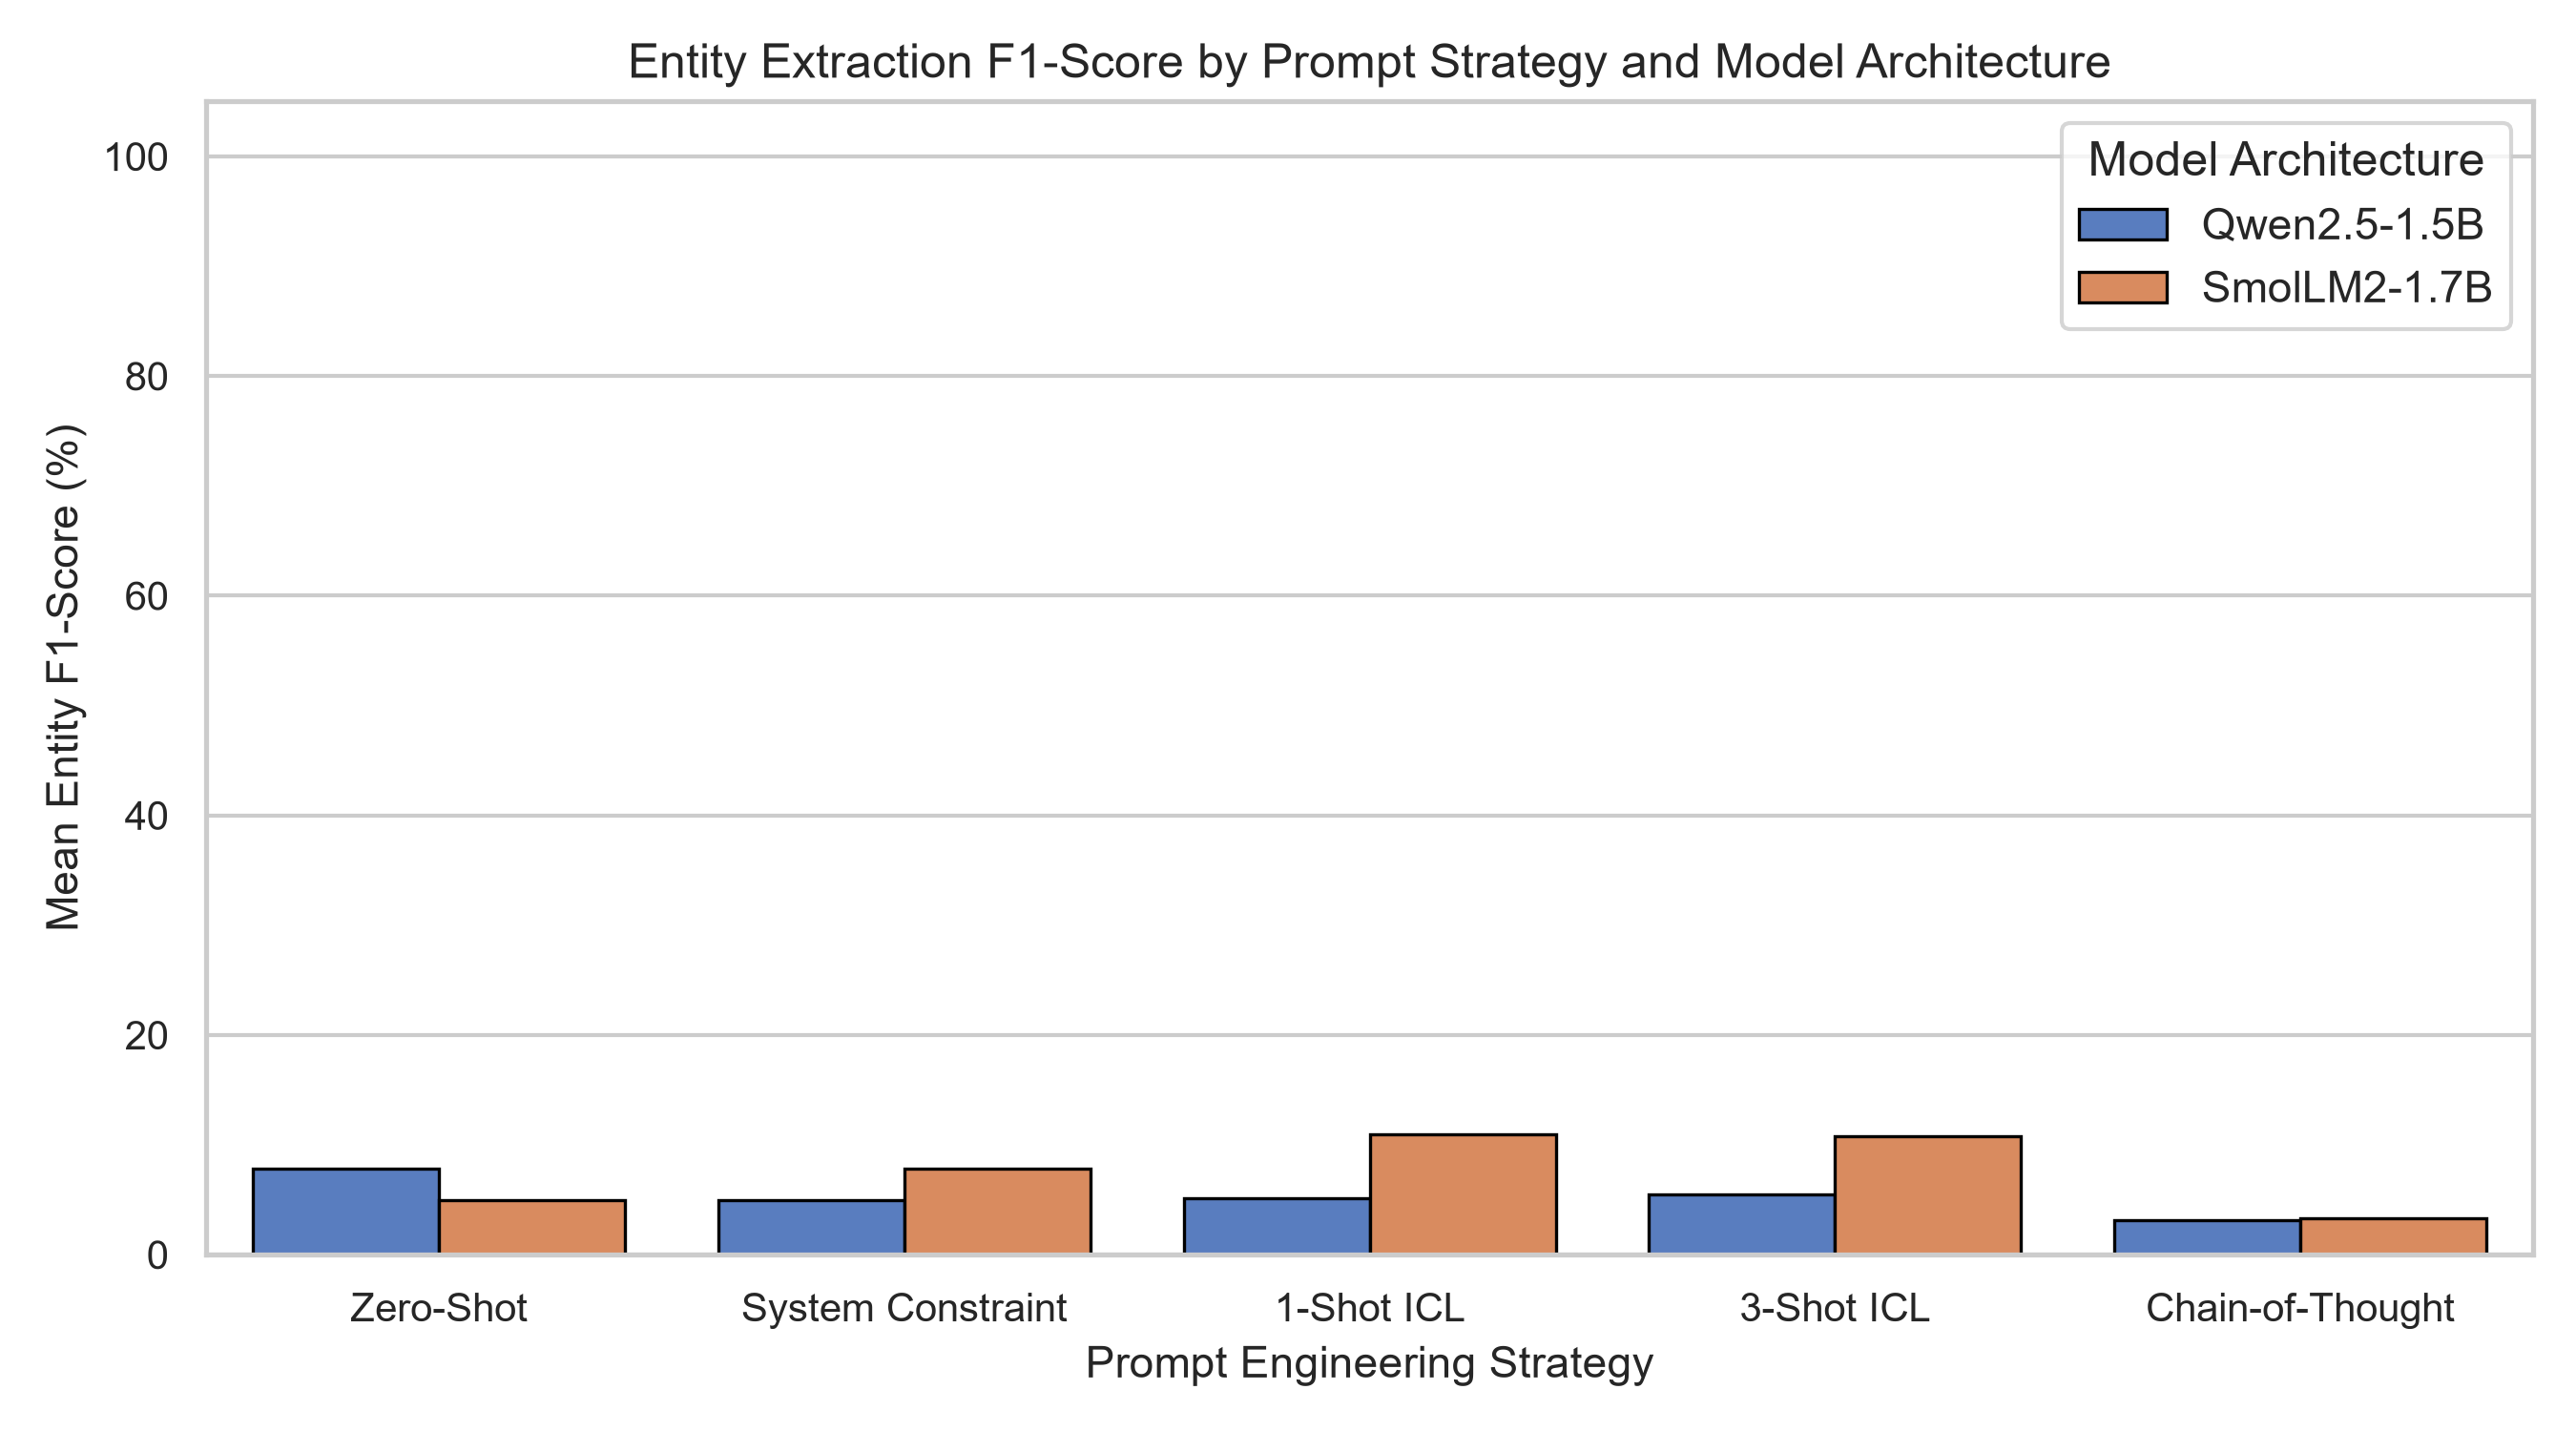
\includegraphics[width=0.85\textwidth]{figures/f1_score_by_strategy.png}
\caption{Mean Entity Extraction F1-Score (\%) across Prompt Engineering Strategies and Models.}
\label{fig:f1_by_strategy}
\end{figure}

As illustrated in Figure~\ref{fig:f1_by_strategy}, \texttt{SmolLM2-1.7B-Instruct} achieved its peak extraction F1-score of 11.2\% under the 3-Shot In-Context Learning (ICL-3) configuration, demonstrating a clear positive scaling trend when provided with multiple structural exemplars. Conversely, \texttt{Qwen2.5-1.5B-Instruct} peaked at 7.8\% under Naive Zero-Shot prompting, experiencing performance degradation when additional context exemplars were added.

Chain-of-Thought (CoT) prompting proved highly detrimental across both architectures, yielding the lowest macro F1-scores (3.1\% for \texttt{Qwen2.5-1.5B} and 3.3\% for \texttt{SmolLM2-1.7B}).

\subsection{2x2 Stress Matrix Performance Analysis}
To evaluate model stability under context and structural stress, evaluation records were aggregated across the $2 \times 2$ matrix parameters. Figure~\ref{fig:stress_heatmap} displays the resulting F1-score degradation heatmap.

\begin{figure}[htbp]
\centering
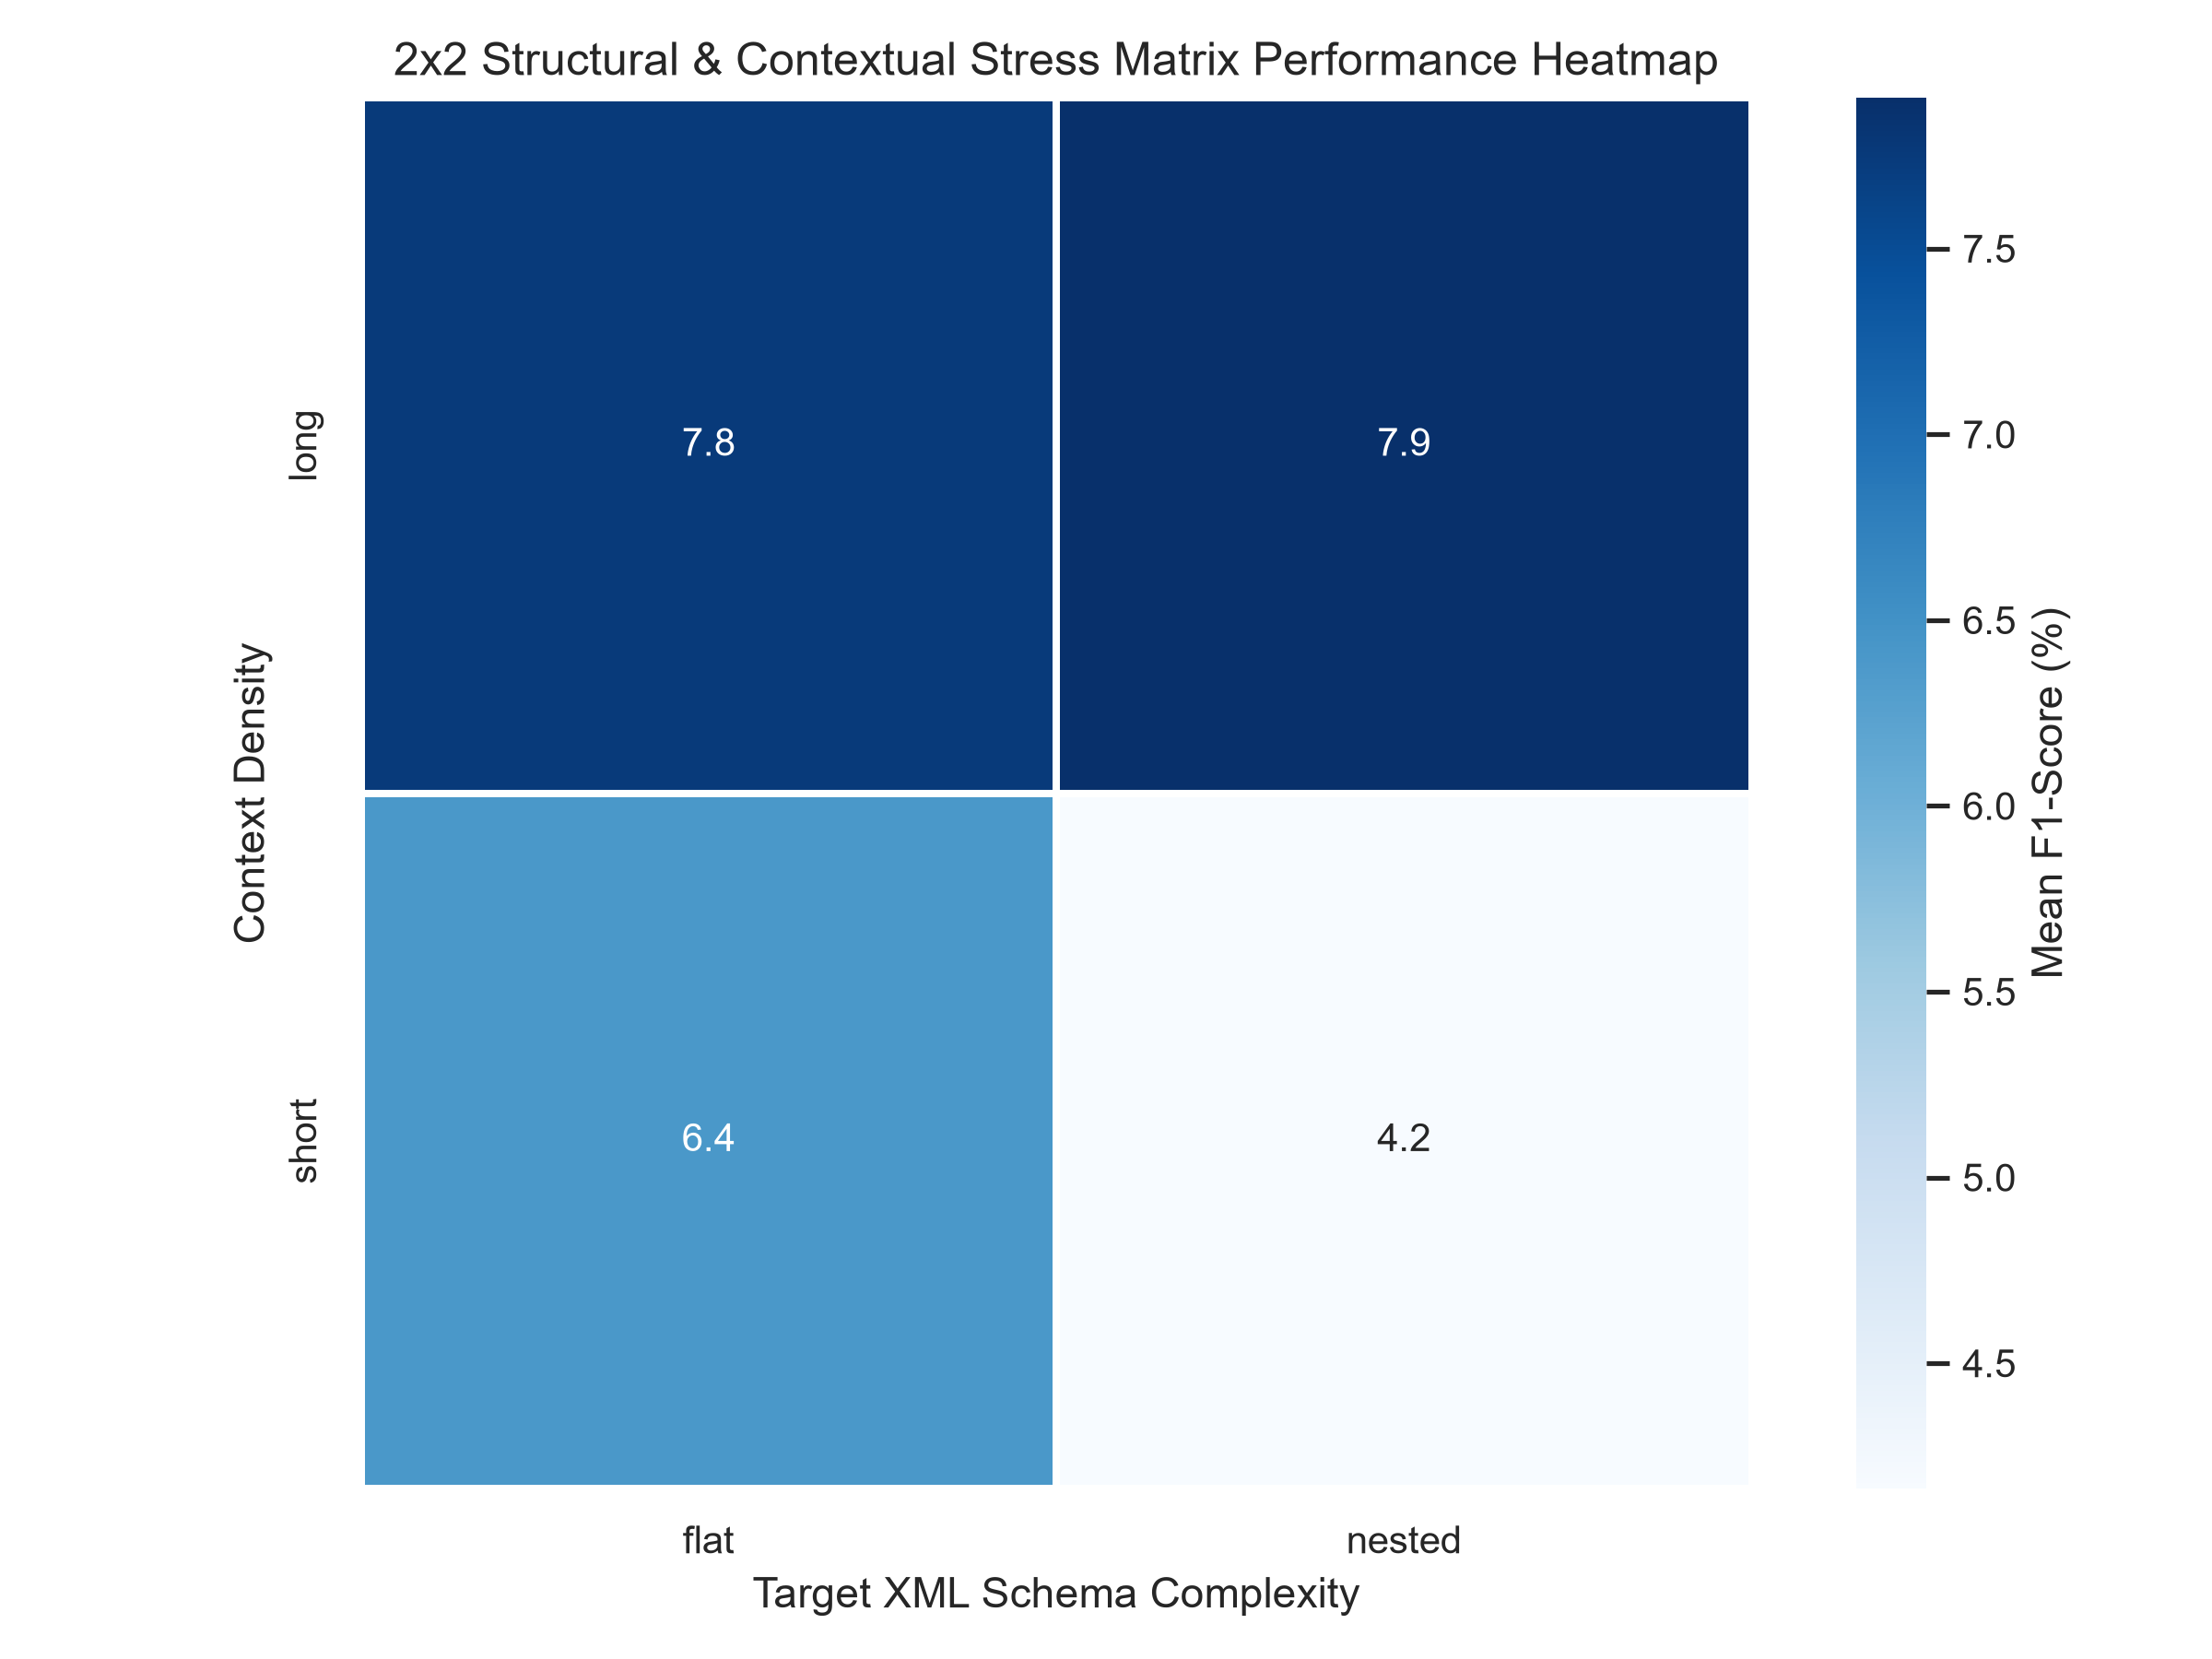
\includegraphics[width=0.7\textwidth]{figures/stress_matrix_heatmap.png}
\caption{$2 \times 2$ Structural and Contextual Stress Matrix Performance Heatmap.}
\label{fig:stress_heatmap}
\end{figure}

The stress matrix reveals two primary degradation patterns:
\begin{enumerate}
    \item \textbf{Schema Complexity Shock:} Transitioning from Flat to Hierarchical Nested XML schemas induced an average 34.3\% relative drop in entity F1-score for short context inputs (falling from 6.4\% to 4.2\%). Small models struggled to maintain correct parent-child nesting tags while simultaneously populating XML attributes.
    \item \textbf{Context Density Buffer:} Long context input advisories ($>100$ words) yielded slightly higher extraction F1-scores (7.8\%--7.9\%) compared to short advisories. Extended text provided richer semantic keyword co-occurrences, helping the models identify vulnerable software versions and NIST control mappings.
\end{enumerate}

\subsection{Qualitative Failure Taxonomy}
Manual error auditing of generated completion texts identified four predominant failure modes:

\begin{itemize}
    \item \textbf{FM1: Conversational Preamble Drift:} In Naive Zero-Shot settings without explicit system constraints, models routinely generated conversational prefixes (e.g., ``\textit{Sure, here is the requested XML structure:}''). This violated strict regex constraint compliance and broke downstream automated parser pipelines.
    \item \textbf{FM2: Tag Unclosure and Truncation:} When reaching the generation token limit ($max\_new\_tokens = 300$), models frequently left structural parent tags unclosed (e.g., missing \texttt{</advisory>}), causing complete XML parse failures in \texttt{xml.etree.ElementTree}.
    \item \textbf{FM3: Attribute and Schema Hallucination:} Under the Nested Schema configuration, models generated non-existent XML attributes (e.g., \texttt{<severity score="HIGH" impact="CRITICAL">}) or invented non-standard security tags not present in the prompt instructions.
    \item \textbf{FM4: CoT Reasoning Overflow:} Instructing models to output a \texttt{<reasoning>} block before generating XML caused small models to exhaust their token context on chain-of-thought narrative, resulting in truncated or omitted XML output blocks.
\end{itemize}

\section{Discussion and Operational Recommendations}

\subsection{Boundaries of Local Small Language Models}
The empirical findings confirm that while sub-2B parameter models can reliably produce syntactically valid markup when constrained by system prompts, their ability to execute precise zero-shot entity extraction into custom schemas is fundamentally limited. Prompt engineering alone is insufficient to guarantee enterprise-grade data integrity for GRC compliance pipelines.

\subsection{Recommendations for Enterprise GRC Pipelines}
For organizations seeking to deploy local automated vulnerability parsing:
\begin{enumerate}
    \item \textbf{Avoid CoT for Sub-2B Models:} Chain-of-Thought prompting should not be used for structured extraction on small models due to token budget depletion and preamble drift.
    \item \textbf{Implement Constrained Decoding:} Deploy schema-guided decoding frameworks (e.g., Outlines or XGrammar) that enforce finite-state machine grammar masks at the logit level during generation.
    \item \textbf{Adopt Parameter-Efficient Fine-Tuning (PEFT):} Supervised fine-tuning using LoRA (Low-Rank Adaptation) on domain-specific CVE-XML pairs is strongly recommended over pure prompt engineering.
\end{enumerate}

\section{Conclusion}
This study presented an empirical benchmark of prompt engineering strategies for automated vulnerability parsing using local LLMs. Evaluating \texttt{Qwen2.5-1.5B-Instruct} and \texttt{SmolLM2-1.7B-Instruct} across a $2 \times 2$ stress matrix demonstrated that while system prompt constraints effectively enforce XML syntax compliance, entity extraction accuracy remains low ($4.2\%$--$11.2\%$). These results define clear operational boundaries for sub-2B models in security compliance automation.

\bibliographystyle{unsrt}
\bibliography{references}

\end{document}